\begin{figure}[H]
\centering
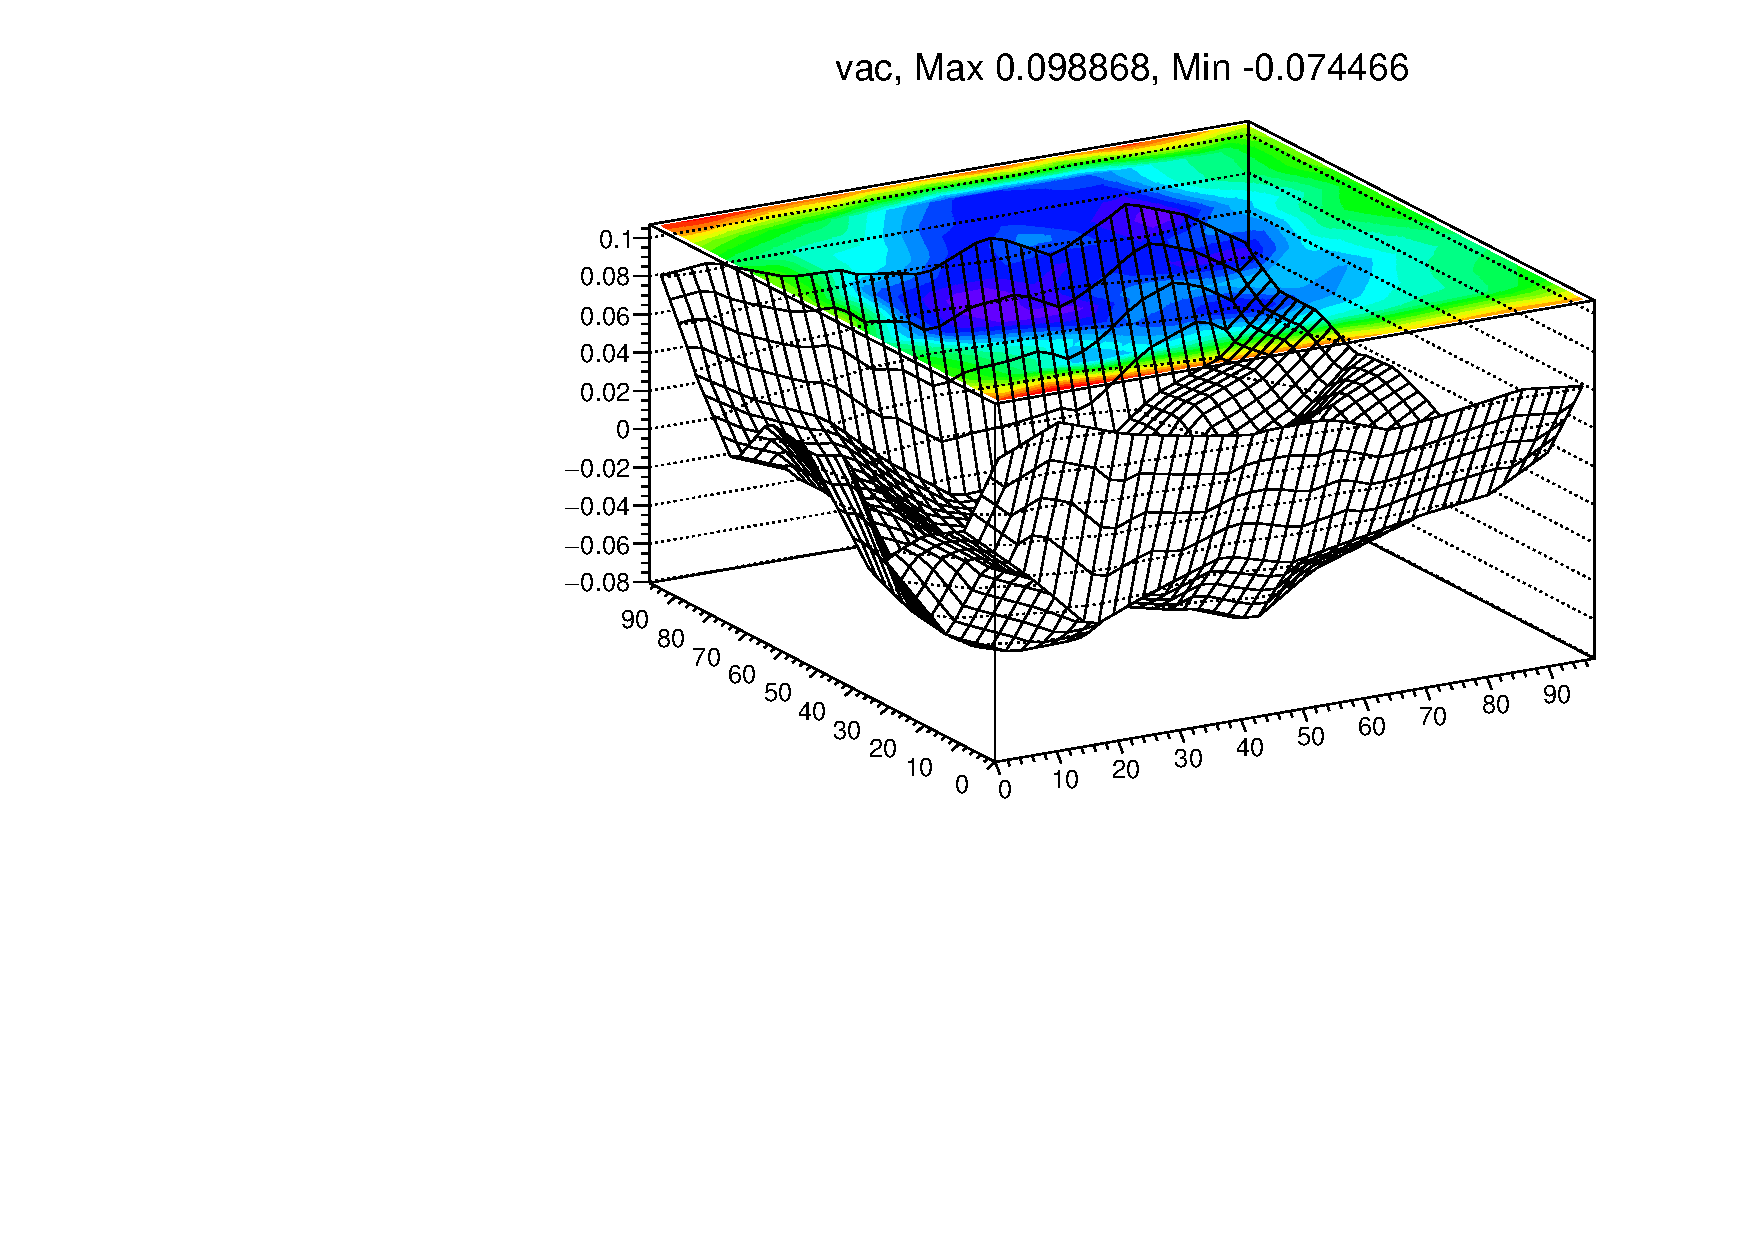
\includegraphics[width=\textwidth]{\FCNCFigures/screenshot/sensorVac.pdf}
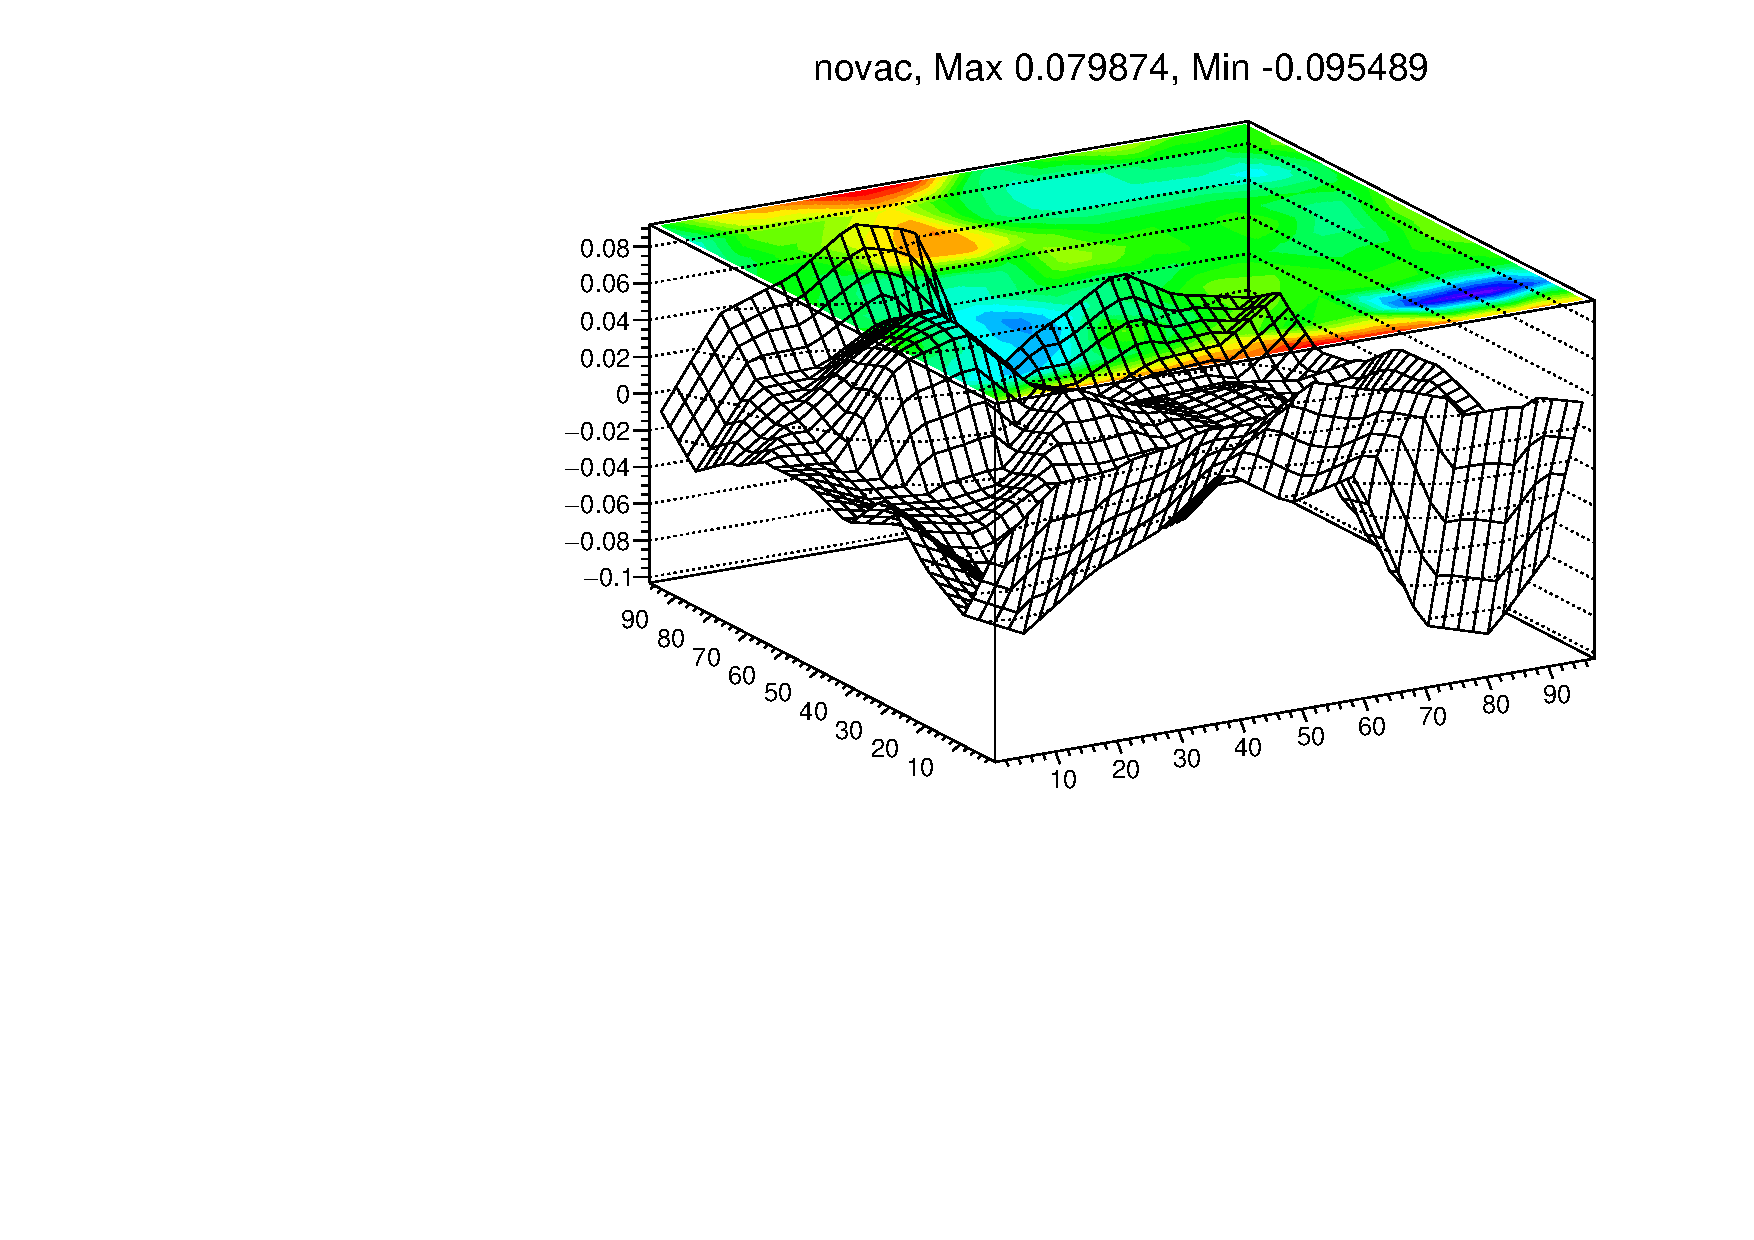
\includegraphics[width=\textwidth]{\FCNCFigures/screenshot/sensorNovac.pdf}
\caption{在使用(左)和不使用(右)真空吸附的时候Sensor的平整程度,对其进行最小二乘,拟合平面,将垂直平面方向的高度差定义为Sensor的弯曲程度。}
\label{fig:sensorVac}
\end{figure}